\chapter*{科学的价值}

\begin{center}
\begin{figure}[h]
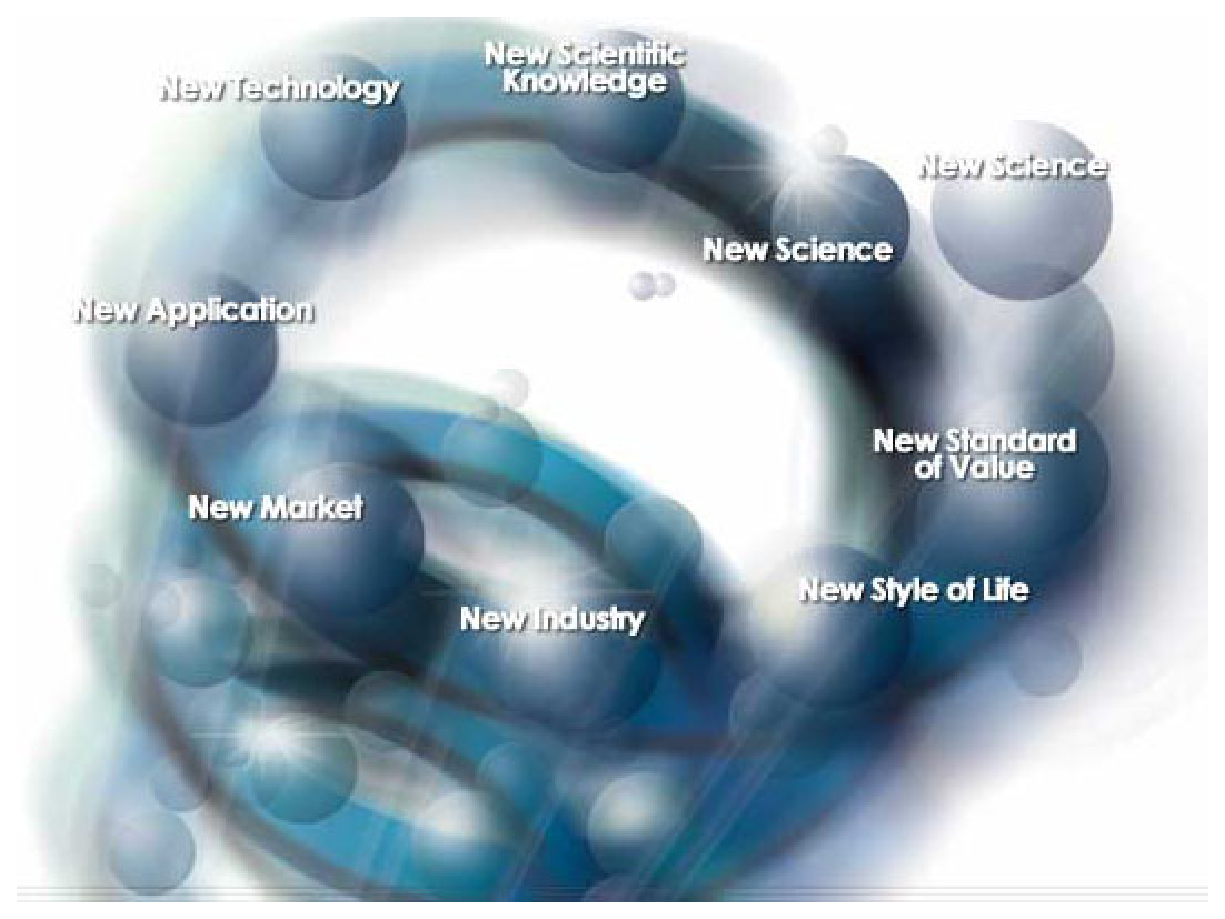
\includegraphics[clip,width=\textwidth]{Foreword/science-vision.ps}
\end{figure}
\end{center}

\begin{quote}
``人类之所以不断的扩展知识和见解,是基于想追究《真理是什么》的结果。
思维和艺术,宗教的不同之处在于是不是用他人都知道的手段去追究真理。
另外,在对真理的追究这一点上,日本语里《科学》的意思和本来的《思维》的意思也有不一样的地方。

新思维生成了新科学[把手段体系化的学问],这种新科学培育了技术和应用,打造了新产业。

新产业生成了人类的新的生活方式,产生了新的价值观,进而生成了新思维。'' 

\qquad 昼马辉夫

\end{quote}


